\subsubsection{Lysets hastighed som en ultimativ hastighed}

Kigger man på den klassiske, ikke-relativistiske mekanik, der er beskrevet af Newtons love, kan en partikel beskrives ved blandt andet dens kinetiske energi, $K$ (også kendt som $E_{\textup{kin}}$), som afhænger af partiklens fart, $v$:
%
\begin{align} \label{rel:eq:KineticEnergy}
    K = \frac{1}{2}m_0v^2.
\end{align}
%
Her er $m_0$ hvilemassen, hvilket er massen af partiklen i det system, hvor partiklen er i hvile, altså i hvilesystemet. Det viser sig nemlig, at det ikke er den samme masse, som hvis partiklen var i bevægelse.

\begin{figure}[t]
    \centering
    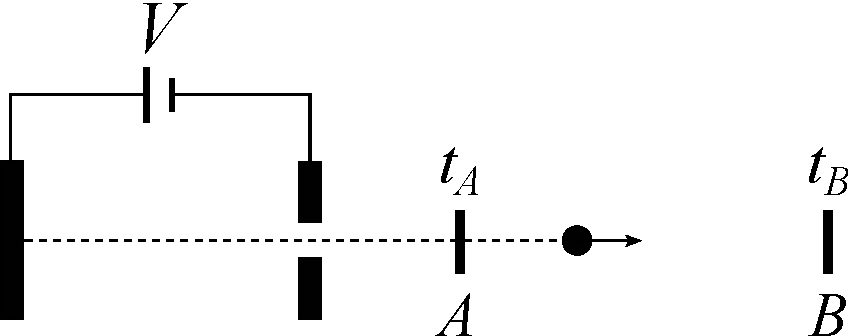
\includegraphics[width=0.5\textwidth]{Rel/RelLorent/EksperimentalSetupElectronVelocity.pdf}
    \caption{En ladet partikel accelereres gennem et spændingsfald $V$ og fortsætter udenfor spændingsfaldet upåvirket (og dermed med konstant hastighed). Partiklens flyvetid mellem to steder A og B måles, og fra dette udregnes partiklens hastighed.}
    \label{fig:ExperimentElectronVelocity}
\end{figure}

Vi ønsker nu at bekræfte udtrykket i \cref{rel:eq:KineticEnergy}, hvorfor vi opstiller et eksperiment, som kan måle hastigheden af en partikel som funktion af dens kinetiske energi. Et sådan eksperiment er skitseret på \cref{fig:ExperimentElectronVelocity}. Her accellereres en elektrisk ladet partikel fra hvile gennem et spændingsfald $V$, således at den opnår den kinetiske energi $K = qV$, hvor $q$ er partiklens ladning. Udenfor spændingsfaldet fortsætter partiklen upåvirket af kræfter, hvorfor den opretholder en konstant fart, $v$. Farten findes ud fra bestemmelse af flyvetiden mellem to punkter, f.eks. $A$ og $B$, hvorimellem længden, $L$, er kendt:
%
\begin{align}
    v &= \frac{L}{t_\textup{B} - t_\textup{A}},
    %
    \intertext{hvor $t_\textup{A}$ og $t_\textup{B}$ er tiden ved punkt $A$ og $B$ respektivt. Måler man nu hastigheden af elektroner på denne måde, og sammenlignes med det klassiske udtryk fra \cref{rel:eq:KineticEnergy}, hvor hastigheden er isoleret (her i enheder af lysets hastighed),}
    %
    \frac{v}{c} &= \sqrt{\frac{2K}{m_0c^2}}, \label{rel:eq:ExpectedExpressionForVelocity}
\end{align}
%
fås \cref{rel:fig:ClassicalVsRelativisticVelocity}.De røde punkter er målepunkter, mens den stiplede sorte kurve angiver det forventede udtryk for $v$ fra \cref{rel:eq:ExpectedExpressionForVelocity}. Overensstemmelsen mellem det forventede udtryk og de målte data er ikke specielt god. I stedet for en liggende parabel, stammende fra kvadratroden i \cref{rel:eq:ExpectedExpressionForVelocity}, flader grafen ud og går øjensynligt mod en grænseværdi på $v/c = 1$, altså $v = c$. Uanset det valgte spændingsfald, så er det altså ikke muligt at drive partiklens hastighed over lysets hastighed, hvilket er et uventet resultat, hvis man følger den Newtonske mekanik. Det kan vises, at det korrekte relativistiske udtryk for en partikels hastighed som funktion af dens kinetiske energi er
%
\footnotetext{At en funktion nærmer sig en grænseværdi asymptotisk, betyder at funktionen kommer uendeligt tæt på, men aldrig rammer helt præcist. Et eksempel på en sådan funktion er $f(x) = e^{-x} = 1/e^x$. Når $x$ går mod uendeligt, er $f(x)$ lig med 1 divideret med noget uendelig stort, hvorfor $f(x)$ må være uendelig lille. $f(x)$ kan aldrig blive præcist lig med nul, men den kan komme uendeligt tæt på, hvorfor man siger at $f(x)$ går asymptotisk mod $0$ for $x \rightarrow \infty$.\label{asymptot}}
%
\begin{align} \label{rel:eq:ExpressionForVelocity}
    v = c \cdot \sqrt{1 - \dfrac{1}{\left(K/m_0c^2 + 1\right)^2}}.
\end{align}
%
Uoverensstemmelsen mellem det klassiske udtryk og de målte værdier på \cref{rel:fig:ClassicalVsRelativisticVelocity} vokser med den kinetiske energi, idet de målte værdier asymptotisk\footref{asymptot} går mod grænseværdien
%
\begin{align} \label{rel:eq:LimitValueForVelocity}
    v_l &\simeq \SI{3.0e8}{\frac{\metre}{\second}}.
\end{align}
%
Denne hastighed overstiger langt de almindelige dagligdagshastigheder, og for små hastigheder, $v \ll c$, er forskellen mellem de målte og klassisk forventede hastigheder forsvindende lille, hvorfor den Newtonske mekanik er god i disse situationer\footnote{Hvis man har lyst til en udfording, kan man bruge teorien om Taylorrækker til at vise, at \cref{rel:eq:ExpressionForVelocity} kan approksimeres med \cref{rel:eq:ExpectedExpressionForVelocity} i grænsen hvor $K/m_0c^2$ er et lille.}. Den klassiske, ikke-relativistiske mekanik bryder altså ikke sammen, men man skal blot overveje, hvornår man opnår så store hastigheder, at de er i det relativistiske område.
%
\begin{figure}[t]
    \centering
    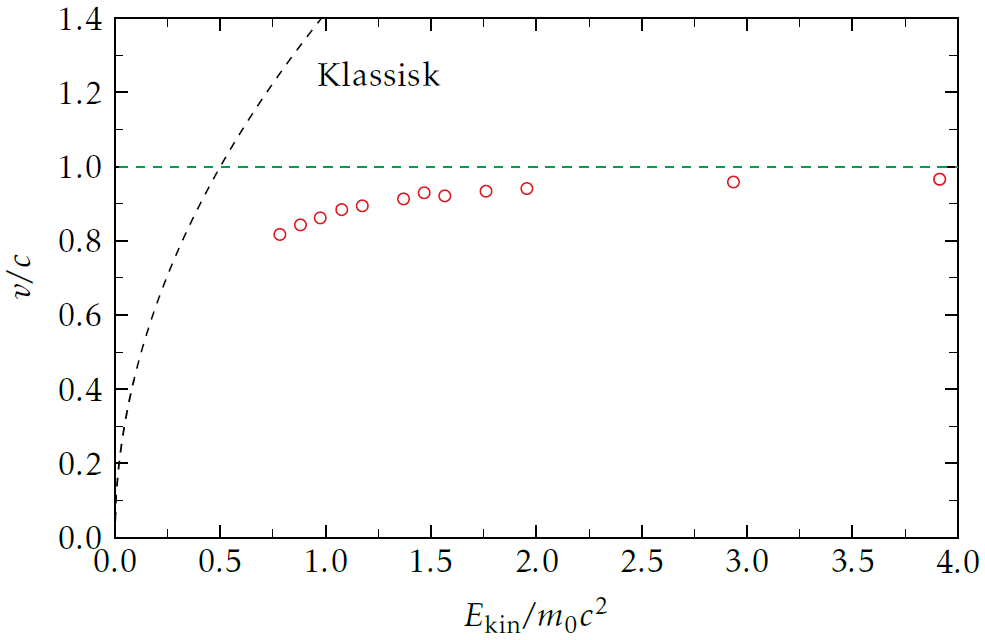
\includegraphics[width=0.7\textwidth]{Rel/RelLorent/ClassicalVsRelativisticVelocityUggerhoej.PNG}
    \caption[]{Hastigheden af elektroner i enheder af lysets hastighed, som funktion af den kinetiske energi i enheder af hvilemasse for en elektron. Den sorte stiplede kurve angiver det klassiske, ikke relativistiske udtryk, de røde punkter er eksperimentelle målepunkter, og den stiplede grønne linje angiver lysets hastighed. Det ses, at de målte værdier asymptotisk\footref{asymptot}~nærmer sig grænseværdien $v = c$, altså kommer $v$ tættere og tættere på $c$ jo større den kinetiske energi bliver. Kilde: figur 5.1 i \cite{uggerhojSpecielRelativitetsteori2016}.}
    \label{rel:fig:ClassicalVsRelativisticVelocity}
\end{figure}

Vi bemærker, at vi kun kender til ét fænomen i naturen, hvis hastighed er lige så stor som $v_l$ fra \cref{rel:eq:LimitValueForVelocity}, hvilket er lysets udbredelse i vakuum:
%
\begin{align}
    c &= \SI{299792458}{\frac{\metre}{\second}},
\end{align}
%
hvilket, indenfor den eksperimentelle usikkerhed af de målinger, der giver grænseværdien, er det samme som grænseværdien.
Det kan konkluderes, at eftersom elektronen er en af de letteste bestanddele af almindeligt stof, med en hvilemasse forskellig fra nul, ikke kan bringes op til lysets hastighed, så må man forvente, at \emph{intet} med en hvilemasse forskellig fra $0$, kan bringes op til denne hastighed.